\subsubsection{Insertion loss/ Streuparameter}\label{subsec:streuparam}

Folgende Theorieabschnitte wurden überwiegend anhand folgender Quellen zusammengestellt: \cite{hftech}.
Die Einfügungsverluste werden analytisch ermittelt. Im ersten Schritt werden die Berechnungen in MATLAB gemacht. Somit können die Funktionen  geplottet werden. Diese Plots werden dann mit Simulationen in MPLAB Mindi verglichen um festzustellen ob diese korrekt sind. Die vollständigen und korrekten Berechnungen können somit in Java implementiert werden. Um die Einfügungsverluste bestimmen zu können, wird das Model der 2-Tore verwendet. Einzelne Schaltungsteile werden in ABCD-Matrixen \ref{ABCD-Matrix} abgebildet, welche dann durch Kaskadierung der einzelnen ABCD-Matrixen zusammengeführt werden. Die Einfügungsverluste werden aus den Streuparameter\ref{subsec:Streuparameter} abgeleitet, welche direkt aus der ABCD-Matrix berechnet werden.
Der S-Parameter S\textsubscript{21} gibt den Transmissionsgrad der Wellen an, die vom Tor 1 zum Tor2 übertragen wird. Die S-Parameter sind abhängig von den Bezugswiderständen (Innenwiderstand der Quelle sowie Lastwiderstand). In unserem Fall sind die Bezugswiderstände mit 50Ohm gegeben.

\begin{equation}\label{equ:Freqgang}
	IL = \left\lvert H(j\omega) \right\rvert = 20*log(\frac{ \left\lvert U_{20} \right\rvert }{ \left\lvert U_2 \right\rvert })
\end{equation}
In der Definition kann das Spannungsverhältnis durch den Streuparameter \ref{subsec:streuparam} (S-Parameter) S\textsubscript{21} ersetzt werden \ref{equ:Einfügungsverluste}.
\begin{equation}\label{equ:Einfügungsverluste}
	IL = -20*log (\left\lvert S_{21} \right\rvert)
\end{equation}
 Dieser Parameter beschreibt den Transmissionsgrad des Filters. Die Einfügungsverluste wären auch mit dem Verhältnis von eingehende zu abegegebene Leistung zu berechnen, jedoch eignet sich diese Methode mehr beim messtechnischen bestimmen der Einfügungsverluste. 
 
 Die Streuparameter (S-Parameter) werden in der Hochfreqeunztechnik verwendet, um das Verhalten von n-Toren zu beschreiben. Bei einem 2-Tor sind vier Streuparameter von nöten um das Verhalten zu beschreiben. Sie beschreiben die Transmission von Tor 1 zu Tor 2, sowie von Tor 2 zu Tor 1. Des weiteren zeigen sie die Reflexion an den Toren auf. Abbildung \ref{fig:2-Tor} \nameref{fig:2-Tor} zeigt die Streuparameter an einem 2-Tor. 
\begin{figure}[H]
	\centering
	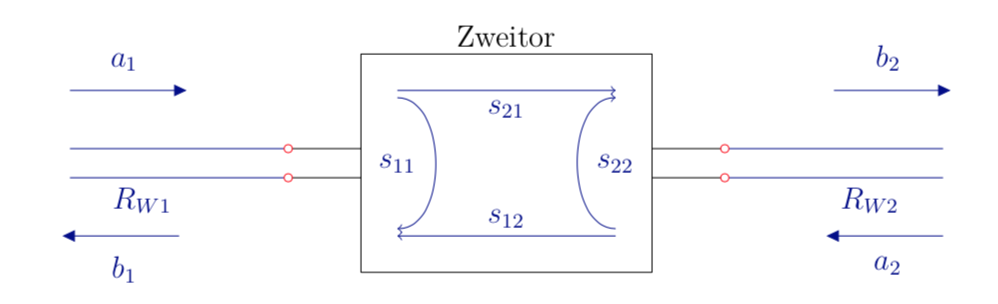
\includegraphics[width=15cm]{s_params_def.png}
	\caption{2-Tor Wellengrössen und Anschlussleitungen \cite{hftech}}
	\label{fig:2-Tor}
\end{figure}
Bei den S-Parameter werden die Eingangs- und Ausgangsgrössen nicht direkt anhand elektrischer Ströme und Spannungen beschrieben. Sie werden mithilfe von Wellengrössen beschrieben, wobei a\textsubscript{i} die einlaufenden Wellen sind und b\textsubscript{i} die Reflektierenden Wellen. Der Index i stellt den Torindex dar. Formel \ref{equ:def_a} und \ref{equ:def_b} zeigen wie die Wellengrössen a\textsubscript{i} sowie b\textsubscript{i} definiert sind.
\begin{equation}\label{equ:def_a}
	a_{ i } = \frac{ U_{ i}+R_{ Wi }I_{ i }}{2*\sqrt{ R_{ Wi } }}
\end{equation}
\begin{equation}\label{equ:def_b}
	b_{ i } = \frac{ U_{ i}-R_{ Wi }I_{ i }}{2*\sqrt{ R_{ Wi } }}
\end{equation}
Die Wellengrössen gelten nur für den gegebenen Bezugswiderstand R\textsubscript{Wi}. Der Bezugswiderstand kann einerseits der Innenwiderstand der angeschlossenen Quelle sein oder der Lastwiderstand der angeschlossenen Last.

Aus der Abbildung 2.3 lässt sich folgende Streumatrix darstellen (Formel \ref{equ:scatteringMatrix}):
\begin{equation}\label{equ:scatteringMatrix}
	\left[
		\begin{matrix}b_1 \\ b_2 \end{matrix}
	\right]
 	=
 	\left[
 		\begin{matrix}
			s_{11}&s_{12} \\s_{21}&s_{22}
		\end{matrix}
	\right]
	* 
	\left[
		\begin{matrix}
			a_1\\b_2
		\end{matrix}
	\right]
\end{equation}
Die Elemente der S-Matrix sind:

\begin{equation}\label{equ:def_s11}
	s_{11} = b_1/a_1\textsf{ Eingangsreflexionsfaktor bei angepasstem Ausgang (a\textsubscript{2}=0)}
\end{equation}
\begin{equation}\label{equ:def_s12}
	s_{12} = b_1/a_2\textsf{ Rückwärtstransmissionsfaktor bei angepasstem Eingang (a\textsubscript{1}=0)}
\end{equation}
\begin{equation}\label{equ:def_s21}
	s_{21} = b_2/a_1\textsf{ Vorwärtstransmissionsfaktor bei angepasstem Ausgang (a\textsubscript{2}=0)}
\end{equation}
\begin{equation}\label{equ:def_s22}
	s_{22} = b_2/a_2\textsf{ Ausgangsreflexionsfaktor bei angepasstem Eingang (a\textsubscript{1}=0)}
\end{equation}
\newpage